\chapter{Showtime}\label{chap:Showtime}

The showtime is the final part of the master project where all groups are presenting their projects and their results.
Before the showtime was beginning a lot of planning was necessary. From the actual presentation and equipment to the brochures and posters everything needed to be planned and organized.

\section{Paperwork}

\subsection{Brochure}

\subsection{Posters}

\subsubsection{Title Poster}
The title poster shows the name of the unplagged master project.

\begin{figure}[!h]
  \centering
  \fbox{
    
\includegraphics[width=0.97\textwidth]{images/poster_title.png}
  }
  \caption{the title poster}
  \label{fig:poster_title}
\end{figure}

\subsubsection{Describing Poster}

Here it is the outlook of the poster which has short describings about the project.

\begin{figure}[!h]
  \centering
  \fbox{
    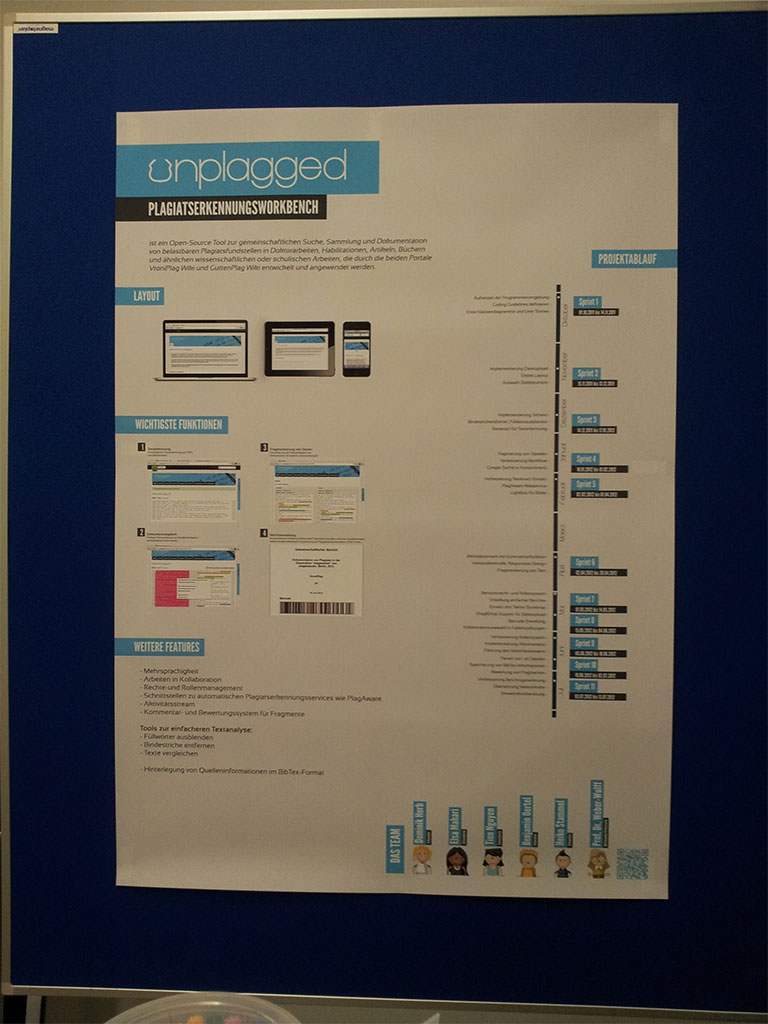
\includegraphics[width=0.97\textwidth]{images/poster_describing.png}
  }
  \caption{the describing poster}
  \label{fig:poster_describing}
\end{figure}

\subsubsection{Technical Poster}


\section{Equipment}
Below there is the list of the equipment which was used for the unplagged exhibition stand.

\begin{itemize}
\item 3 iMacs
\item 3 tables
\item 2 higher tables
\item 3 pinboards
\item 2 floodlights
\end{itemize}

\section{Outlook of the exhibition stand}
Below there are some snapshots of the unplagged exhibition stand.





